\documentclass[a4paper,twoside,12pt]{scrbook}
%% === nezbytné balíčky:
\usepackage[T1]{fontenc}    % kódování písma
%\usepackage[IL2]{fontenc}  % kódování písma

\usepackage[utf8]{inputenc}     % vstupní znaková sada tohoto dokumentu: UTF-8
%\usepackage[cp1250]{inputenc}  % vstupní znaková sada tohoto dokumentu: Windows 1250
%\usepackage[latin2]{inputenc}  % vstupní znaková sada tohoto dokumentu: ISO Latin 2
\DeclareUnicodeCharacter{2029}{ }

\usepackage[czech]{babel} % česky psaná práce, typografická pravidla. Překládejte pomocí "latex.exe" nebo "pdflatex.exe"
%\usepackage{czech} % česky psaná práce. Překládejte pomocí "pdfCSlatex.exe" ("cslatex.exe" asi bude mít problém s balíkem geometry)

\usepackage[a4paper, hmarginratio=3:2]{geometry} % využití A4 stránky a nastavení okrajů (u vazby bude širší)

\usepackage{pdfpages} % pokud nemáte formulář "Zadání bak./dipl. práce" naskenovaný jako PDF, tak ZAKOMENTUJTE
\usepackage[hidelinks]{hyperref} % v PDF budou klikací odkazy ("hidelinks" je nebude rámovat)

%% === balíčky, které se mohou hodit:
%\usepackage{encxvlna} % postará se o spojky a předložky, které dle českých pravidel nesmí být na konci řádku. Dokumentace: http://texdoc.net/texmf-dist/doc/generic/encxvlna/encxvlna.pdf (chová se správně k "vnitřku" listings?)

\usepackage{graphicx} % balíček pro vkládání rastrových grafických souborů (PNG apod.)
%\usepackage{epsfig} % balíčky pro vkládání grafických souborů typu EPS
%\usepackage{float} % rozšířené možnosti umístění obrázků

%\usepackage{caption} % pro popisky obrázků, tabulek atd.

\usepackage{tabularx} % rozšířené možnosti tabulek
%\usepackage{tabu} % jiný balík pro rozšířené možnosti tabulek

% \usepackage{listings}  % balíček vhodný pro ukázky zdrojového kódu v~textu práce/příloh. Nutno nastavit! http://ftp.cvut.cz/tex-archive/macros/latex/contrib/listings/listings.pdf
\usepackage{amsmath} % balíček pro pokročilou matematickou sazbu
%\usepackage{color} % pro možnost barevného textu
%\usepackage{fancybox} % umožňuje pokročilé rámečkování

%\usepackage{index} % nutno použít v případě tvorby rejstříku balíčkem makeindex
%\newindex{default}{idx}{ind}{Rejstřík} % zavádí rejstřík v případě použití balíku index
\usepackage{amssymb}
\usepackage[nice]{nicefrac}

\usepackage{minted}
\renewcommand{\listingscaption}{Ukázka kódu}
\renewcommand{\listoflistingscaption}{Seznam ukázek kódu}

\frenchspacing % za větou bude mezislovní mezera (v anglických textech je mezera za větou delší)
\widowpenalty=1000 % "síla" zákazu vdov (= jeden řádek ze začátku odstavce na konci stránky)
\clubpenalty=1000 % "síla" zákazu sirotků (= jeden řádek/slovo z konce odstavce samostatně na začátku stránky)
\brokenpenalty=1000 % "síla" zákazu zlomu stránky za řádkem, který má na konci rozdělené slovo

\topmargin=-15mm      % horní okraj trochu menší
\textwidth=150mm      % šířka textu na stránce
\textheight=240mm     % "výška" textu na stránce


\pagenumbering{arabic} % číslování stránek arabskými číslicemi
\pagestyle{plain}      % stránky číslované dole uprostřed

\parindent=0pt % odsazení 1. řádku odstavce
\parskip=7pt   % mezera mezi odstavci

\newcommand{\ti}{\textit} % zkrácený příkaz pro kurzívu
\newcommand{\tb}{\textbf} % zkrácený příkaz pro tučné písmo

\DeclareMathOperator*{\argmax}{arg\,max}
\DeclareMathOperator*{\argmin}{arg\,min}

%% --- zde jsou zavedeny některé "konstanty" - některé musíte změnit! --- %%
\newcommand{\cvut}{České vysoké učení technické v~Praze}
\newcommand{\fjfi}{Fakulta jaderná a fyzikálně inženýrská}
\newcommand{\ksi}{Katedra softwarového inženýrství}
\newcommand{\program}{Aplikace přírodních věd} % změňte, pokud máte jiný stud. program
\newcommand{\obor}{Aplikace softwarového inženýrství} % změňte, pokud máte jiný obor

\newcommand{\druh}{Výzkumný úkol} % nebo "Diplomová práce"
\newcommand{\woman}{} % pokud jste ŽENA, ZMĚŇTE na: ...{\woman}{a} (je to do Prohlášení)

\newcommand{\logoCVUT}{
\includegraphics{symbol_cvut_konturova_verze_cb.pdf}} % logo ČVUT -- podle grafického manuálu ČVUT platného od prosince 2016. Pokud nevyhovuje PDF-verze, tak použijte jinou variantu loga: https://www.cvut.cz/logo-a-graficky-manual -> "Symbol a logo ČVUT v Praze"). Pokud chcete logo úplně vynechat, zadejte místo "\includegraphics{...}" text "\vspace{35mm}"

% přesně podle formuláře "Zadání bak./dipl. práce" VYPLŇTE:
\newcommand{\nazevcz}{Webový systém pro testování znalostí studentů}    % český název práce (přesně podle zadání!)
\newcommand{\nazeven}{}          % anglický název práce (přesně podle zadání!)
\newcommand{\autor}{Bc. František Navrkal}   % vyplňte své jméno a příjmení (s akademickým titulem, máte-li jej)
\newcommand{\vedouci}{Ing. Martin Plajner} % vyplňte jméno a příjmení vedoucího práce, včetně titulů, např.: Doc. Ing. Ivo Malý, Ph.D.
\newcommand{\pracovisteVed}{Ústav teorie informace a automatizace, Akademie věd České republiky} % ZMĚŇTE, pokud vedoucí Vaší práce není z KSI
\newcommand{\konzultant}{--} % POKUD MÁTE určeného konzultanta, NAPIŠTE jeho jméno a příjmení
\newcommand{\pracovisteKonz}{--} % POKUD MÁTE konzultanta, NAPIŠTE jeho pracoviště

% podle skutečnosti VYPLŇTE:
\newcommand{\rok}{2017}  % rok odevzdání práce (jen rok odevzdání, nikoli celý akademický rok!)
\newcommand{\kde}{Praze} % studenti z Děčína ZMĚNÍ na: "Děčíně" (doplní se k "prohlášení")

% \newcommand{\klicova}{Klíčová slova}   % zde NAPIŠTE česky max. 5 klíčových slov
% \newcommand{\keyword}{Key words}       % zde NAPIŠTE anglicky max. 5 klíčových slov (přeložte z češtiny)
\newcommand{\abstrCZ}{Popis práce česky}    % zde NAPIŠTE abstrakt v češtině (cca 7 vět, min. 80 slov)
% \newcommand{\abstrEN}{Popis práce anglicky} % zde NAPIŠTE abstrakt v angličtině

\newcommand{\prohlaseni}{Prohlašuji, že jsem svůj výzkumný úkol vypracoval\woman{} samostatně a použil\woman{} jsem pouze podklady (literaturu, projekty, SW atd.) uvedené v přiloženém seznamu.} % text prohlášení můžete mírně upravit :-)

\newcommand{\podekovani}{Děkuji Ing. Martinu Plajnerovi za jeho pomoc a ochotu.} % NAPIŠTE poděkování, např. svému vedoucímu:
% Děkuji Ing. Eleonoře Krtečkové, Ph.D. za vedení mé bakalářské práce a za podnětné návrhy, které ji obohatily.
% NEBO:
% Děkuji vedoucímu práce doc. Pafnutijovi Snědldítětikaši, Ph.D. za neocenitelné rady a pomoc při tvorbě bakalářské práce.


\begin{document}
%%%%%%%%%%%% TITULNÍ STRANA -- na následujících cca 30 řádků NESAHEJTE!!!  Generuje se AUTOMATICKY %%%%%%%%%%%%
\thispagestyle{empty}

\begin{center}
	{\LARGE
		\cvut\par
		\fjfi
	}
    \vspace{10mm}

    \begin{tabular}{c}
		\tb{\ksi} \\[3pt]
		\tb{Obor: \obor}\\
    \end{tabular}

   \vspace{10mm} \logoCVUT \vspace{15mm}

   {\huge \tb{\nazevcz}\par}
   \vspace{5mm}
   {\huge \tb{\nazeven}\par}

   \vspace{15mm}
   {\Large \MakeUppercase{\druh}}

   \vfill
   {\large
    \begin{tabular}{ll}
    Vypracoval: & \autor\\
    Vedoucí práce: & \vedouci\\
    Rok: & \rok
    \end{tabular}
   }
\end{center}

\clearpage{\pagestyle{empty}\cleardoublepage} % prázdná stránka za tou "titulní", bez čísla

%%%%%%%%%%%% ZADÁNÍ PRÁCE %%%%%%%%%%%%
% Zadání (podepsané děkanem!) musíte NASKENOVAT. Ideálně jako 2stránkové PDF (soubor "zadani_cele.pdf").
% Před svázáním to v jednom výtisku VYMĚNÍTE ZA ORIGINÁLNÍ ZADÁNÍ (podepsané děkanem fakulty)!
\newpage  % SEM NESAHEJTE!
\thispagestyle{empty} % SEM NESAHEJTE!

%% zde podle toho, jak jste zadání naskenovali, VYBERTE variantu A, B nebo C:
%
% --- varianta A: zadání naskenované jako 2stránkové PDF:
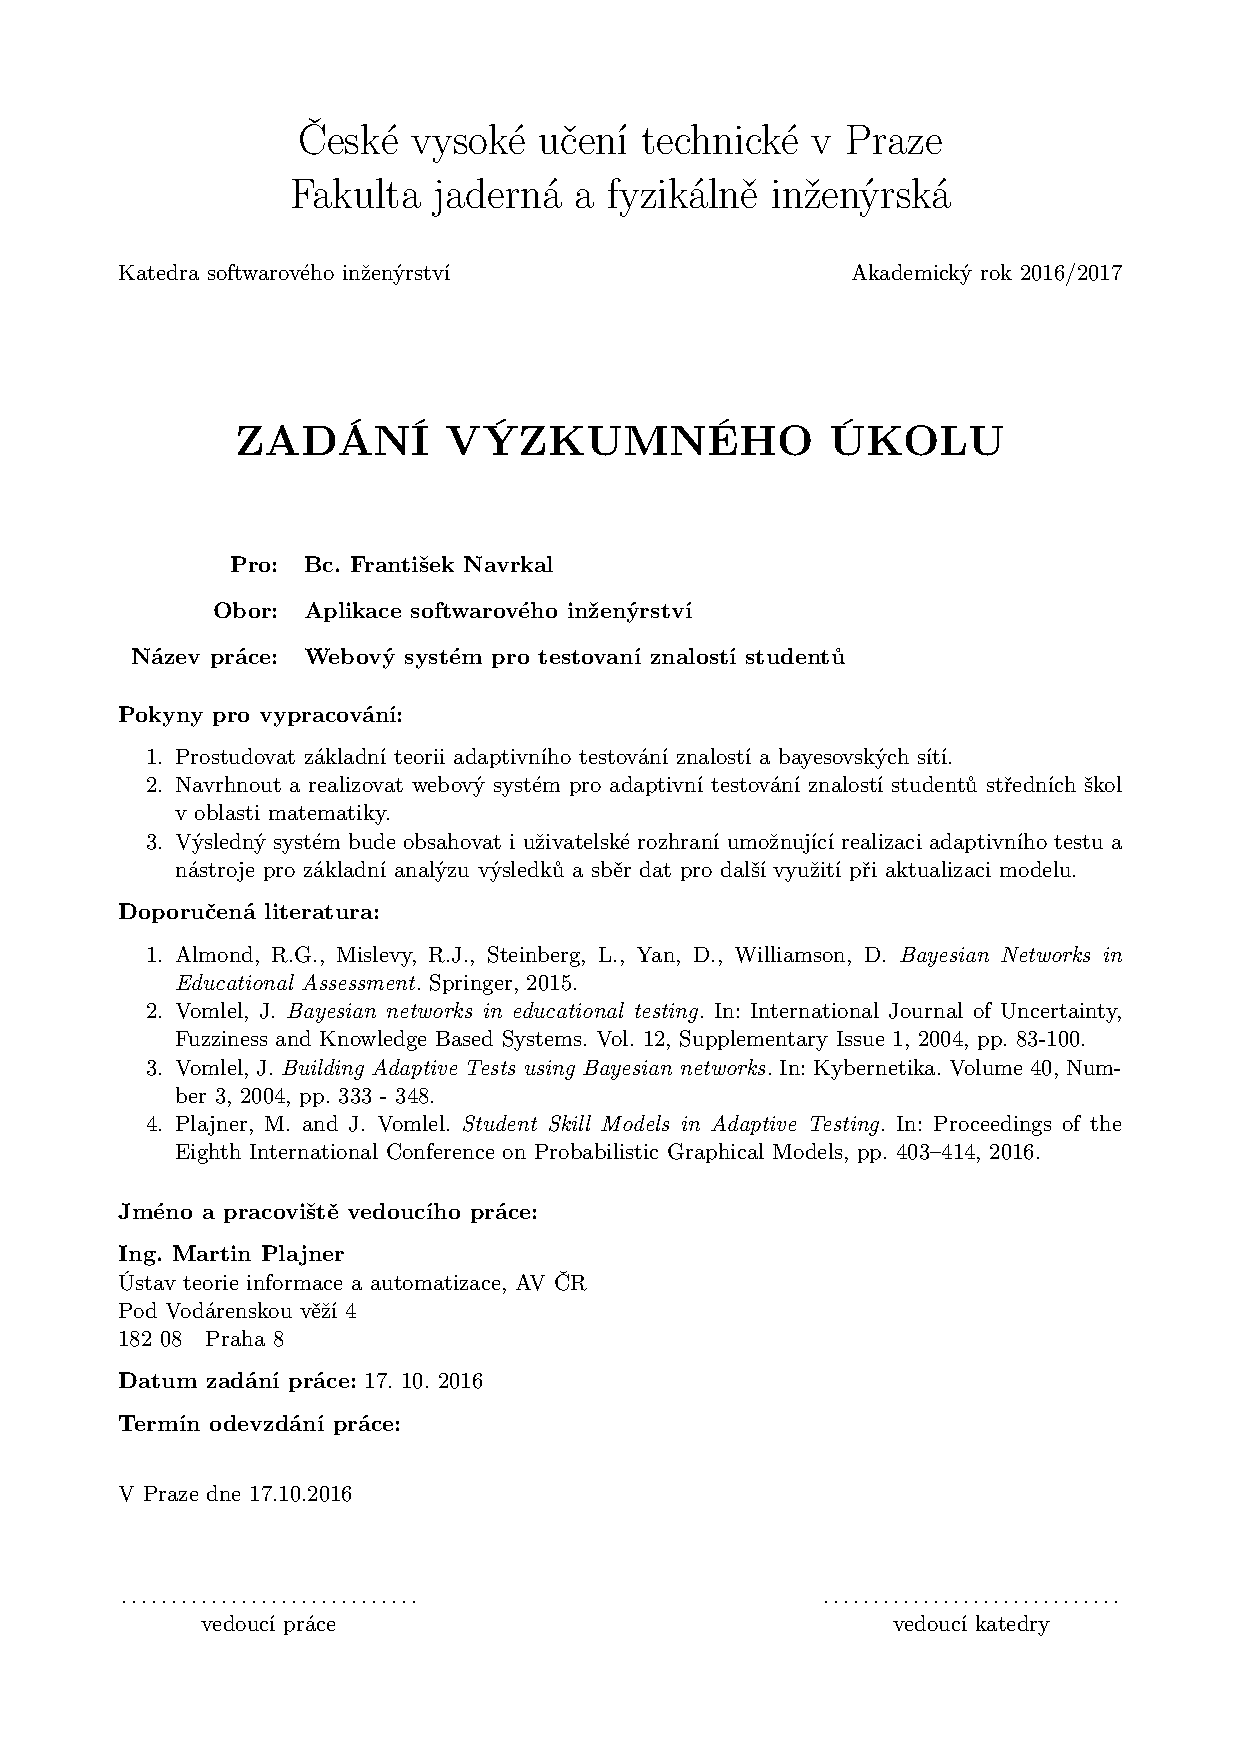
\includepdf{zadani_cele.pdf} % NAHRAĎTE správným souborem!
%
%% --- varianta B: zadání naskenované jako jednotlivé stránky:
%\includepdf[pages={1}]{zadani1.pdf} % 1. strana zadání v PDF
%\includepdf[pages={1}]{zadani2.pdf} % 2. strana zadání v PDF
%
%% --- varianta C: zadání naskenované jako 2 samostatné obrázky:
%% 1. strana zadání
%\begin{center}
%     \includegraphics[width=1\textwidth]{zadani1.jpg}
%\end{center}
%% 2. strana zadání
%\newpage  % SEM NESAHEJTE!
%\thispagestyle{empty} % SEM NESAHEJTE!
%\begin{center}
%     \includegraphics[width=1\textwidth]{zadani2.jpg}
%\end{center}

\newpage % SEM NESAHEJTE!
\thispagestyle{empty}  % SEM NESAHEJTE!

~ % SEM NESAHEJTE!

%%%%%%%%%%%% Prohlášení -- SEM NESAHEJTE! Generuje se automaticky z výše nastavených maker \kde{} a \prohlaseni{}. %%%%%%%%%%%%
\newpage % SEM NESAHEJTE!
\thispagestyle{empty}  % SEM NESAHEJTE!

~ % SEM NESAHEJTE!
\vfill % prázdné místo. SEM NESAHEJTE!

\tb{Prohlášení} % SEM NESAHEJTE!

\vspace{1em} % vertikální mezera. SEM NESAHEJTE!
\prohlaseni

\vspace{2em}  % SEM NESAHEJTE!
\hspace{-0.5em}\begin{tabularx}{\textwidth}{X c}  % SEM NESAHEJTE!
V \kde\ dne .................... &........................................ \\	% SEM NESAHEJTE!
	& \autor
\end{tabularx}	% SEM NESAHEJTE!


%%%%%%%%%%%% Poděkování  %%%%%%%%%%%%
\newpage
\thispagestyle{empty}

~
\vfill % prázdné místo


% -- následující kus kódu (do "%%%%%%%%%%%% ABSTRAKT") můžete odstranit, pokud nechcete psát poděkování:
\tb{Poděkování}

\vspace{1em} % vertikální mezera
\podekovani
\begin{flushright}
\autor
\end{flushright}  % <------- tady končí stránka s poděkováním


%%%%%%%%%%%% ABSTRAKT atp. Je generován AUTOMATICKY podle maker nastavených na začátku souboru) %%%%%%%%%%%%
% \newpage   % SEM NESAHEJTE!
% \thispagestyle{empty}   % SEM NESAHEJTE!
%
% % příprava:    (na následujících 8 řádků NESAHEJTE!)
% \newbox\odstavecbox
% \newlength\vyskaodstavce
% \newcommand\odstavec[2]{%
%     \setbox\odstavecbox=\hbox{%
%          \parbox[t]{#1}{#2\vrule width 0pt depth 4pt}}%
%     \global\vyskaodstavce=\dp\odstavecbox
%     \box\odstavecbox}
% \newcommand{\delka}{120mm} % šířka textů ve 2. sloupci tabulky
%
% % použití přípravy:    % dovnitř "tabular" vůbec NESAHEJTE!
% \begin{tabular}{ll}
%   {\em Název práce:} & ~ \\
%   \multicolumn{2}{l}{\odstavec{\textwidth}{\bf \nazevcz}} \\[1em]
%   {\em Autor:} & \autor \\[1em]
%   {\em Studijní program:} & \program \\
%   {\em Obor:} & \obor \\
%   {\em Druh práce:} & \druh \\[1em]
%   {\em Vedoucí práce:} & \odstavec{\delka}{\vedouci\\ \pracovisteVed} \\
%   {\em Konzultant:} & -- %\odstavec{\delka}{\konzultant \\ \pracovisteKonz}  % VYMAŽTE text "-- %" v případě, že jste neměli konzultanta
%  \\[1em]
%   \multicolumn{2}{l}{\odstavec{\textwidth}{{\em Abstrakt:} ~ \abstrCZ  }} \\[1em]
%   {\em Klíčová slova:} & \odstavec{\delka}{\klicova} \\[2em]
%
%   {\em Title:} & ~\\
%   \multicolumn{2}{l}{\odstavec{\textwidth}{\bf \nazeven}}\\[1em]
%   {\em Author:} & \autor \\[1em]
%   \multicolumn{2}{l}{\odstavec{\textwidth}{{\em Abstract:} ~ \abstrEN  }} \\[1em]
%   {\em Key words:} & \odstavec{\delka}{\keyword}
% \end{tabular}



%%%%%%%%%%%% Obsah práce ... je generován AUTOMATICKY %%%%%%%%%%%%
\cleardoublepage  % SEM NESAHEJTE!
\parskip=0pt
\tableofcontents % SEM NESAHEJTE!
\parskip=7pt
% \newpage % SEM NESAHEJTE!


%--------------------------------------------------------
%|         Zde začíná SAMOTNÁ PRÁCE (text)              |
%--------------------------------------------------------

% \cleardoublepage
\chapter*{Úvod} % SEM NESAHEJTE!
\addcontentsline{toc}{chapter}{Úvod} % SEM NESAHEJTE!
%
V první kapitole tohoto textu je krátce představen koncept počítačového adaptivního testování a jedna z cest jeho implementace, konkrétně pomocí bayesovských sítí. Toto krátké představení by mělo poskytnout dostatečný znalostní základ pro aspoň obecné pochopení fungování konkrétního systému popsaného v kapitole druhé.

Druhá kapitola zároveň slouží jako obecná dokumentace webové aplikace pro adaptivní testování v rámci výzkumného úkolu vyvíjené. V této kapitole jsou také popsány možnosti dalšího vývoje aplikace.

Na samotném konci tohoto textu jsou jako jediná příloha uvedeny instrukce pro instalaci a nasazení aplikace.
%
%\input{vnitrek_uvod.tex}

%---------------------------------------
\chapter{Adaptivní počítačové testování}
% \cleardoublepage
% \section{Adaptivní testování}
Adaptivní počítačové testování je způsob získávání informací o znalostech studenta, při kterém se průběh testování mění na základě informací získaných v jeho průběhu (nebo i před jeho zahájením). V anglicky psané literatuře se pro toto používá označení computerized adaptive testing (CAT). Využití adaptivního testování umožňuje kombinovat výhody individuálního testování jako zvýšená přesnost a úspora času i námahy testovaného s možností hromadného testování. \cite{almond_tlustospis}%vypsat zde publikace ze kterých v sekci čerpám

\subsection{Motivace}
V \cite[strana~10]{Wainer2000} je uveden následující argument. Hromadně aplikovaný test musí, aby fungoval dobře pro širokou škálu úrovní jednotlivých měřených dovedností, obsahovat otázky různé obtížnosti. Pokud by na příklad neobsahoval lehké otázky, nemohl by test přesně měřit nízkou úroveň příslušných dovedností.

Tento fakt ovšem znamená, že zdatný student ve statickém testu musí nejdříve odpovědět na mnoho pro něj jednoduchých otázek, než se dostane k otázkám, které mají nějakou vypovídací hodnotu o jeho dovednostech. Toto vede k mrhání času a námahy studenta, přináší to též do procesu testování nechtěné faktory jako chyby z nedbalosti způsobené nudou.

V případě, že je úroveň měřených dovedností studenta naopak nízká, hrozí zase zmatek, frustrace a nekvalitní data, pokud slabý student správnou odpověď jen náhodou uhodne.


\subsection{Průběh adaptivního testování}

Samotný průběh adaptivního testování sestává z opakování těchto kroků: \cite{plajner16}
\begin{enumerate}
	\item Výběr otázky na základě modelu znalostí studenta dle zvoleného výběrového kritéria.
	\item Zobrazení otázky studentovi, získání odpovědi a její vyhodnocení.
	\item Vložení získaných informací do modelu znalostí studenta a jeho aktualizace.
	\item Kontrola ukončovacích kritérií a případné ukončení testu při jejich dosažení.
\end{enumerate}
Celý jeden cyklus těchto kroků zde bude uváděn jako krok celého testu.

Tomuto ovšem musí předcházet tvorba celého testu a příslušného modelu znalostí. Po sběru dat o dostatečném vzorku průběhů testování lze na jejich základě zvýšit přesnost (resp. prakticky prediktivní schopnost) modelu. Příklad obého je uveden v sekci \ref{sec:test_design}. %odkazat se na další text, vysvětlit víc konkrétně již zde
%
% \subsection{Části adaptivního modelu}
% Pro adaptivní testování je nutno
% \begin{itemize}
% 	\item samotného obsahu testu, tedy
% \end{itemize}


% -------------------------------------------------

\section{Znalostní model (bayesovské sítě)}
Pro modelování znalostí studenta v rámci přístupu k adaptivnímu testování použitému v této práci (navrženému v \cite{almond_tlustospis}) se používá bayesovských sítí. Jedná se o pravděpodobnostní grafický model popisující vztahy mezi náhodnými veličinami pomocí rozdělení podmíněné pravděpodobnosti.

\subsection{Formální definice}
Bayesovskou síť pro naše účely můžeme definovat formálně jako uspořádanou dvojici orientovaného acyklického grafu $B_S = (V,E)$ (tzv. struktura sítě), kde každému prvku $i \in V$ odpovídá náhodná veličina $X_i$, a množiny $B_P$  funkcí $P(X_i\,|\,(X_j)_{j\in pa(i)})$, které udávají podmíněné pravděpodobnostní rozdělení $X_i$ v závislosti na hodnotě veličin odpovídajících (přímým) předchůdcům (neboli rodičům) $i$ v $B_S$ značeným jako $pa(i)$. (Toto značení je možná trochu zavádějící v případě uzlů bez předchůdců, tedy u nichž $pa(i) = \emptyset$, tam totiž vlastně nejde o podmíněné pravděpodobnosti, ale pravděpodobnosti nepodmíněné.) Množinu všech náhodných veličin budu značit $\mathcal{X}=\{X_i\,|\,i \in V\}$.

V dále uvažovaných případech budou $X_i$ nabývat jen určitých diskrétních hodnot (stavů veličiny) z množin $\mathbb{X}_i$, takže si prvky $B_P$ můžeme také představovat jako funkce zobrazující vektor stavů předchůdců $i$ v $B_S$ na vektor pravděpodobností stavů $X_i$. Prakticky lze takovouto funkci zapsat jako tak zvanou tabulku podmíněných pravděpodobností. (Opět nemusí jít nutně o pravěpodobnosti podmíněné.)

\subsection{Neformální popis}
Bayesovské sítě popisují kauzální vztahy mezi pozorovanými náhodnými veličinami. V našem případě půjde kauzální vztah mezi odpověďmi studenta na otázky v testu a jeho měřenými dovednostmi.

Teoreticky by bylo možné uvažovat všechny možné konjunkce stavů uvažovaných náhodných veličin $\mathbb{X}$ a popsat jejich pravděpodobnostní rozdělení, ale počet možných konjunkcí je dán jako součin počtu stavů jednotlivých veličin:
\begin{equation}
	\label{eq:conjunctions_cardinality}
	|\mathbb{X}| = \prod_{\mathbb{X}_i \in \{\mathbb{X}_i\,|\,i \in V\}} \left|\mathbb{X}_i\right|,
\end{equation}
což je v praktických případech (stačí již s řádově desítkami veličin) často astronomické číslo, protože minimální smysluplný počet možných stavů náhodné veličiny jsou 2, což znamená, že $\mathbb{X}$ bude vždy aspoň $2^{\left|\mathcal{X}\right|}$.

Toto je důvod, proč se uvažují jen určité možné kauzální vztahy mezi pozorovanými veličinami, konkrétně ty, jejichž přítomnost odhadl buď učící algoritmus na základě sesbíraných dat nebo expert na danou problematiku.

Tyto vztahy jsou pak kvantifikovány opět buďto expertem nebo algoritmicky na základě dat. Konkrétně jsou určeny funkce v $B_P$, tedy speciálně příslušné tabulky podmíněných pravděpodobností. Metody učení tabulek podmíněných pravděpodobností jsou popsány na příklad v \cite[kapitola~9]{almond_tlustospis}.

Třeba v případě popisovaném v sekci \ref{sec:test_design} autoři použili smíšený přístup: struktura sítě (tedy kvalitativní popis kauzálních vztahů) byla odhadnuta experty (samotnými autory) a tabulky podmíněných pravděpodobností (kvantitativní popis) pak byly naučeny algoritmicky na základě sesbíraných dat.

% Jeden z předpokladů pro běžné výpočty v bayesovských sítích je, že pro každou veličinu $X_i$ platí, že je podmíněně nezávislá na veličinách, které  \textbf{ne}jsou reprezentovány jejími potomky v síti, podmíněno znalostí stavu veličin reprezentovaných jejími předky v síti. Zkráceně: každá veličina je podmíněně nezávislá na svých nepotomcích podmíněno znalostí svých předků.

% Tento požadavek v praxi nelze striktně splnit, protože by model musel pokrýt opravdu všechny předpoklady pro správné zodpovězení otázek. Modely se tedy snaží pokrýt jen ty nejvíce relevantní a nejlépe měřitelné. Komplexita zamýšlených modelů také značně zvyšuje nároky na sběr dat pro jejich návrh. % rozpracovat nebo zahodit

\subsection{Příklady}
\label{sec:net_examples}
V \cite{almond_tlustospis} je hned v úvodu jako příklad uvedena síť na obrázku \ref{fig:almond_BN_example}. Uzly s kroužky udávají jednotlivé dovednosti (čtení, psaní, poslech, mluvení) a uzly s trojúhelníky udávají stavy vyhodnocení úkolů vyžadujících jednotlivé kombinace těchto dovedností.

\begin{figure}
  \centering
    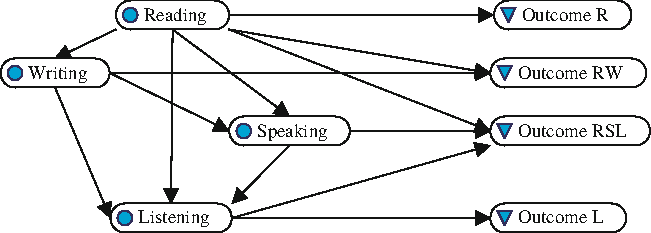
\includegraphics[width=0.8\textwidth]{almond_BN_example.pdf}
  \caption{Příklad bayesovské síťě z \cite{almond_tlustospis}.}
  \label{fig:almond_BN_example}
\end{figure}

Další příklad jsem vybral z \cite{plajner16}. Na obrázku \ref{fig:complex_BN_plajner16} zelené uzly reprezentují jednotlivé dovednosti a žluté uzly otázky. Uzel \emph{S8} (celková dovednost, konkrétně znalost jednoduchých funkcí) je předchůdcem všech uzlů, následují ostatní zelené uzly (jednotlivé prvky celkové dovednosti: znalost polynomů, exponenciálních funkcí a tak dále) a na konec žluté uzly, které reprezentují jednotlivé úlohy v testu.

\begin{figure}
  \centering
    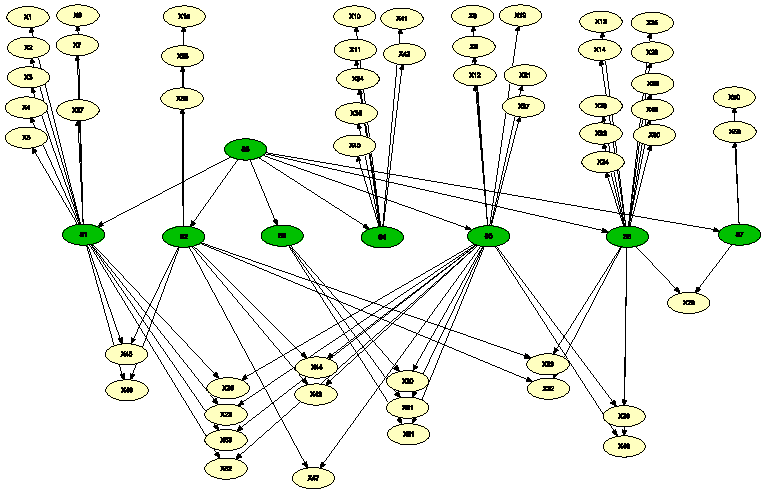
\includegraphics[width=0.85\textwidth]{complex_BN_plajner16.pdf}
  \caption{Příklad bayesovské síťě z \cite{plajner16}.}
  \label{fig:complex_BN_plajner16}
\end{figure}

\subsection{Dovednosti a otázky}
Množina všech náhodných veličin $\mathcal{X}$ se ve zde blíže probíraných případech bude typicky dělit na 2 disjunktní podmnožiny $\mathcal{S} \cup \mathcal{Q} = \mathcal{X}$, kde $\mathcal{S}$ je množina veličin představujících dovednosti a $\mathcal{Q}$ otázky (je tomu tak v obou zmíněných příkladech a předpkládám to i ve své webové aplikaci). Dále ještě mohou být v bayesovské síti zastoupeny jako náhodné veličiny další informace o studentovi jako třeba věk, pohlaví nebo výsledky jiného testování.

Vyhodnocení adaptivního testu bude v následujícím textu znamenat určení pravděpodobnostní rozdělení veličin z $\mathcal{S}$ na základě získaných dat. (Toto lze studentovi prezentovat jako pravděpodobnosti dosažené úrovně jeho znalostí, případně možná přístupněji třeba pomocí určitého odvozeného skóre a podobně.)

Množinu $\mathcal{Q}$ ještě budeme někdy dělit na další 2 disjunktní podmnožiny $Q = \widehat{\mathcal{Q}} \cup \overline{\mathcal{Q}}$, kde $\widehat{\mathcal{Q}}$ je množina dosud nezodovězených otázek a $\overline{\mathcal{Q}}$ již zodpovězených.

\subsection{Aktualizace modelu v průběhu testování}
Informace získané v průběhu testování se do modelu vkládají tak, že se rozdělení veličiny z $\mathcal{Q}$ na základě odpovědi na příslušnou otázku testu nahradí rozdělením, kde je jeden ze stavů již jistý (tedy vektor pravděpodobnostní stavů je pak vektor obsahující jeden prvek s hodnotou 1 a všechny ostatní s hodnotou 0). Toto umožní aktualizaci rozdělení ostatních veličin jak z $\mathcal{S}$, tak z $\widehat{\mathcal{Q}}$.

Formálně budu psát, že nějaká $X_i \in \overline{\mathcal{Q}}$ nabývá hodnoty $x_i \in \mathbb{X}_i$ jako $X_i = x_i$. Případně k rozlišení nahradím $X_i$ za $S_i$ nebo $\mathbb{X}_i$ za $\mathbb{Q}_i$ a podobně.

% --------------------------------------

\section{Návrh adaptivního testu}
\label{sec:test_design}
Možností, jak navrhnout test je nespočet. Pro představu krátce shrnu jako příklad článek podrobně popisující návrhu testu, konkrétně \cite{vomlel_plajner2015}.

\subsection{Návrh obsahu a sběr dat}
Nejdříve autoři navrhli statický test, ten předložili malé skupině studentů. Na základě zpětné vazby studentů pak vytvořili další, pro studenty srozumitelnšjší, návrh, ze kterého byly také odebrány otázky, které se ukázaly neefektivní pro zisk informací.

Test nakonec obsahoval 29 úloh, které se dále rozdělily celkem na 53 podúloh. Úlohy byly alternativně vyhodnocovány pomocí bodového ohodnocení, nebo jen jako správně či špatně vypracované.

Sběru dat se celkem zúčastnilo 281 studentů. O těchto studentech si autoři sesbírali také některá jejich osobní data jako věk, pohlaví, jméno a jejich známky z matematiky, chemie a fyziky za poslední 3 pololetí.


\subsection{Srovnání znalostních modelů}
V článku autoři porovnali celkem 14 různých modelů, které se lišily mj. počtem uvažovaných stavů náhodných veličin, počtem měřených dovedností a zahrnutím osobních dat studentů.

Struktura sítě byla vždy pro daný srovnávaný model pevná (navržená na základě předpokladů autorů článku o příslušných kauzálních vztazích). Tabulky podmínených pravděpodobností se vždy v rámci desetinásobné křížové validace odhadly (naučily) na základě $\nicefrac{9}{10}$ náhodně vybraných případů (učící množiny). Jednotlivé modely pak byly porovnávány na základě chování modelu v simulacích na zbývající $\nicefrac{1}{10}$ případů (testovací množině).

Modely autoři konkrétně porovnávali na základě míry úspěšnosti odhadu hodnocení zatím v simulaci neřešených úloh na základě úloh již v dané simulaci vyřešených a vyhodnocených, to celé v závislosti na počtu vyřešených úloh (počtu odsimulovaných kroků testování). Za odhad se bral nejpravděpodobnější stav dané zatím neřešené úlohy v danému kroku testu.

Jako kritérium výběru úlohy v simulacích autoři použili maximalizaci středního informačního zisku (neboli poklesu entropie) stavu dovedností po vyhodnocení kandidátní úlohy. (Podrobně rozebráno v podsekci \ref{subsec:information_gain}.)

\subsection{Vyhodnocení}
Autoři došli k tomu, že příliš jednoduché modely si nevedly dobře -- ukázalo se jako výhodné uvažovat raději 3 než pouze 2 stavy u dovednostních veličin.

Zahrnutí osobních údajů o studentovi do modelu vylepšilo úspěšnost předpovědí jen v počátečních krocích testování, poté měly pouze malý pozitivní, nebo dokonce negativní efekt.

Složitější z modelů pravděpodobně postihl tak zvaný over-fitting, to jest naučené tabulky podmíněných pravděpodobností nezobecňovaly dobře vztahy z učící množiny pro testovací množinu, takže si nakonec nevedly dobře.

V jejich novějším článku \cite{plajner16} používají autoři mj. síť na obrázku \ref{fig:complex_BN_plajner16}, která se liší od té z \cite{vomlel_plajner2015} hlavně přidáním souhrné dovednostní veličiny jako předchůdce všech ostatních veličin. Tato síť měla hlavně ve spojení s jejich novým algoritmem pro učení z testovací množiny mnohem lepší úspěšnost předpovědí.

\begin{figure}
  \centering
    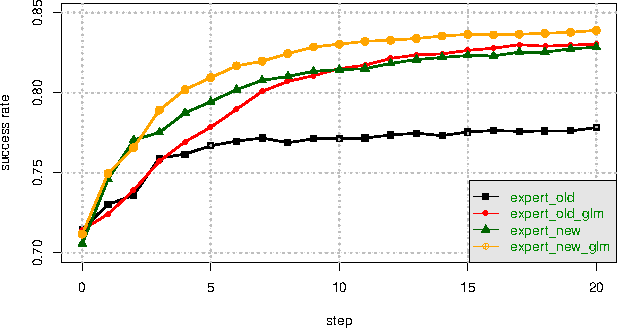
\includegraphics[width=0.85\textwidth]{comparison_chart_plajner16.pdf}
  \caption{Srovnání úspěšnosti znalostních modelů z \cite{plajner16}. Modely \texttt{expert\_old(\_glm)} jsou modely se strukturou bez uzlu celkové dovednosti, \texttt{expert\_new(\_glm)} jsou modely s ní. Přípona \texttt{\_glm} značí jinou metodu učení tabulek podmíněných pravděpodobností.}
  \label{fig:comparison_chart_plajner16}
\end{figure}

% -------------------------------------

\section{Strategie výběru otázek}
\label{sec:question_selection}
Na základě znalostního modelu se mohou v průběhu adaptivního testování vybírat otázky k zobrazení studentovi dle různých kritérií. Uvedu zde příklady jednoduchých \uv{hladových} stragií srovnávaných v \cite{question_selection} určených pro bayesovské modely znalostí a poté nastíním i možné jiné, komplikovanější, strategie.

Nechť již zodpovězené otázky nabývají hodnot $e=\{Q_i=q_i|Q_i\in\overline{\mathcal{Q}}\}$, pak lze vybrat otázku na příklad následujícími způsoby.

\subsection{Maximalizace středního informačního zisku}
\label{subsec:information_gain}
Toto kritérium je motivováno tím, že jako výsledek testu chceme co nejvíce snížit nejistotu ve stavech $S_i \in S$. Hledáme tedy otázku $\widehat{Q}^*_i \in \widehat{\mathcal{Q}}$, jejíž vyhodnocení tuto nejistotu co nejvíce sníží ve smyslu střední hodnoty dle pravděpodobnosti odpovědí na ní. Nejistotu zde měříme pomocí Shannonovy entropie, konkrétně:
\begin{equation}
	H(e) = -\sum_{S_i \in \mathcal{S}}\sum_{s_i \in \mathbb{S}_i}P(S_i=s_i|e) \log{}P(S_i=s_i|e),
\end{equation}
po zodpovězení uvažované otázky $\widehat{Q}_i \in \widehat{\mathcal{Q}}$ a jejím vyhodnocení na stav $\widehat{Q}_i = \widehat{q}_i$ tedy:
\begin{equation}
	H(e, \widehat{Q}_i = \widehat{q}_i) = -\sum_{S_i \in \mathcal{S}}\sum_{s_i \in \mathbb{S}_i}P(S_i=s_i|e, \widehat{Q}_i = \widehat{q}_i) \log{}P(S_i=s_i|e, \widehat{Q}_i = \widehat{q}_i).
\end{equation}

Střední hodnota entropie na dovednostech po nějaké odpovědi na $\widehat{Q}_i$ bude tedy:
\begin{equation}
	EH(\widehat{Q}_i,e) = \sum_{\widehat{q}_i \in \widehat{\mathbb{\mathcal{Q}}}_i}P(\widehat{Q}_i = \widehat{q}_i|e) H(e, \widehat{Q}_i = \widehat{q}_i).
\end{equation}

Toto kritérium vybírá otázku $\widehat{Q}^*_i$ jako:
\begin{equation}
	\widehat{Q}^*_i = \argmax_{\widehat{Q}_i \in \widehat{\mathcal{Q}}} H(e) - EH(\widehat{Q}_i,e).
\end{equation}

\subsection{Maximalizace středního rozptylu stavů dovedností}
Použití tohoto kritéria ve zde rozebrané podobě předpokládá, že veličiny dovedností $S_i$ jsou binární, tedy mohou nabývat pouze dvou hodnot. Konkrétně zde budou tyto hodnoty značeny jako $0$ v případě absence dovednosti a $1$ v případě, že student danou dovednost má.

Toto kritérium se snaží o dobrou separaci studentů na základě jejich dovedností. Konkrétně jde o tuto hodnotu:
\begin{equation}
	var(\mathcal{S}|e, \widehat{Q}_i) = \sum_{S_i \in \mathcal{S}}\sum_{\widehat{q}_i \in \widehat{\mathbb{Q}}_i} \left(P(S_i=1|e) - P(S_i=1|e, \widehat{Q}_i = \widehat{q}_i) \right)^2 P(\widehat{Q}_i = \widehat{q}_i|e).
\end{equation}

Nakonec se analogicky jako u předchozího kritéria vybere $\widehat{Q}^*_i$ jako:
\begin{equation}
	\widehat{Q}^*_i = \argmax_{\widehat{Q}_i \in \widehat{\mathcal{Q}}} var(\mathcal{S}|e, \widehat{Q}_i).
\end{equation}

\subsection{Maximalizace středního rozptylu stavů otázek}
Uvedená podoba tohoto kritéria vyžaduje, aby byly binární tentokrát veličiny otázek $Q_i$. Zcela analogicky:
\begin{equation}
	var(\widehat{Q}_i|e) = \sum_{s \in \mathbb{S}_{pa(i)}} \left(P(\widehat{Q}_i=1|e) - P(\widehat{Q}_i=1|e, s) \right)^2 P(s|e),
\end{equation}
kde $\mathbb{S}_{pa(i)}=\{S_j=s_j\,|\,j\in pa(i),\, s_j\in\mathbb{S}_j\}$ je množina všech možných konjunkcí stavů těch dovednostních veličin v $\mathcal{S}$, jejichž uzly jsou předchůdci uzlu $i$ dané otázky v síti. Stavy ostatních dovednostních veličin není třeba uvažovat, neboť jsou tak zvaně d-separované (koncept vysvětlen názorně třeba v \cite[strana 26 až 32]{Jensenc2007}).

$\widehat{Q}^*_i$ se vybere předvídatelně jako:
\begin{equation}
	\widehat{Q}^*_i = \argmax_{\widehat{Q}_i \in \widehat{\mathcal{Q}}} var(\widehat{Q}_i|e).
\end{equation}

Pokud by k výpočtu $var(\widehat{Q}_i|e)$ bylo nutné uvažovat příliš mnoho konjunkcí stavů dovedností (jejichž počet by udával vzorec \ref{eq:conjunctions_cardinality}, kde by množina $\mathbb{X}$ byla nahrazena $\mathbb{S}_{pa(i)}$), bylo by možné použít následující aproximaci:
\begin{equation}
	var^*(\widehat{Q}_i|e) = \sum_{S_i \in \mathcal{S}_{pa(i)}}\sum_{s_i \in \mathbb{S}_i} \left(P(\widehat{Q}_i=1|e) - P(\widehat{Q}_i=1|e, S_i = s_i) \right)^2 P(S_i = s_i|e).
\end{equation}
Tato aproximace byla použita i pro dosažení výsledků na obrázku \ref{fig:question_selection_comparison}.

\subsection{Srovnání a komplexnější strategie}

\begin{figure}
  \centering
    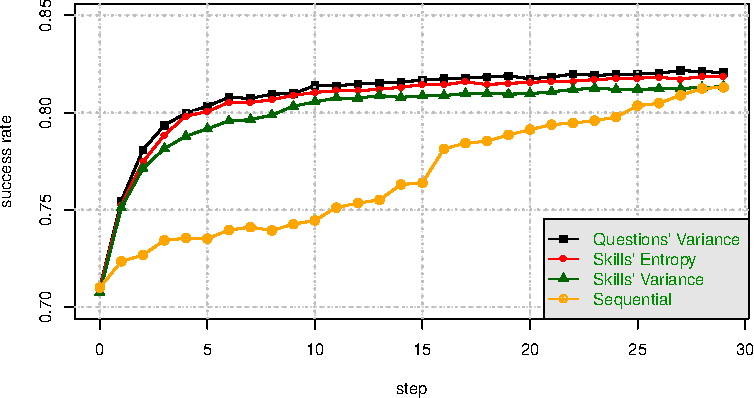
\includegraphics[width=0.85\textwidth]{question_selection_comparison.pdf}
  \caption{Srovnání úspěšnosti kritérií výběru otázky z \cite{question_selection}.}
  \label{fig:question_selection_comparison}
\end{figure}

Případ porovnání zmíněných metod výběru je na obrázku \ref{fig:question_selection_comparison}. Srovnávané strategie jsou \uv{hladové}, konkrétně uvažují vždy jen jeden krok testu dopředu.

Šlo by ovšem též simulovat všechny možné scénáře vývoje testu několik kroků dopředu, vyčíslit hodnoty maximalizovaného kritéria na konci těchto simulací a poté přiřadit každé kandidátní otázce $\widehat{Q}_i \in \widehat{\mathcal{Q}}$ příslušnou střední hodnotu kritéria napříč scénáři, které by mohly následovat zodpovězení uvažované otázky. Tento proces je podrobně rozebrán v \cite{vomlel_building} včetně praktických heuristik pro zrychlení výpočtů.

% -------------------------------------

\chapter{Vyvíjená systém}
V této kapitole je popsán samotná aplikace, kterou jsem v rámci výzkumného úkolu vyvíjel. Moje aplikace tvoří uživatelské rozhraní pro knihovnu vyvíjenou na Ústavu teorie informace a automatizace AV ČR, která zajišťuje ve zde rozebírané webové aplikaci samotné výpočty na příslušné bayesovské síti, zvané \textit{Computerized Adaptive Testing Generic Framework} (dále jen \texttt{catest}).

Všechny cesty v souborovém systému v této kapitole jsou uvedeny relativně vůči kořenu složky \texttt{CArisTotle}. Doporučuji během čtení této kapitoly paralelně procházet kód v repozitáři na \url{https://github.com/FNj/CArisTotle}.

\section{Výběr nástrojů}
Vedoucí práce mě upozornil na systém \textit{R Shiny}  \cite{r_shiny}. Jedná se o knihovnu psanou v jazyce \textit{R} \cite{R}, ve kterém je psaná i samotná knihovna \texttt{catest}. Já zase přišel s nápadem použít jako jádro aplikace \uv{microframework} (aplikační rámec) \textit{Flask}  \cite{flask} psaný v \textit{Pythonu}  \cite{python}.

Systém \textit{R Shiny} je ovšem cílen na různé datově analytické výstupy spíše než na obecnější webové aplikace, také mám opravdu jen malé zkušenosti s programovacím jazykem \textit{R}, ve kterém je tento systém napsaný. Raději jsem tedy nakonec zůstal u \textit{Pythonu} a \textit{Flasku}, se kterým mám jak ze školního, tak profesionálního prostředí asi největší zkušenosti ze všech programovacích jazyků. \textit{Python} je také mnohem více uzpůsoben multiparadigmatickému programování (porovnáváno třeba v \cite{multiparadigm}).

Protože takto používám kombinaci dvou různých programovacích jazyků, je nutné mít k dispozici nějaké rozhraní mezi nimi. Původně jsem uvažoval o úplně vlastním řešení, ale nakonec jsem našel knihovnu \textit{RPy2} \cite{rpy2}, která mi tvorbu rozhraní velmi usnadnila.

Aplikace musí ukládat dlouhodobě informace o uživatelích, definicích adaptivního testu a průběhu jednotlivých případů testování. Tyto jsou ukládány do relační databáze pomocí knihovny \textit{SQLAlchemy} \cite{sqlalchemy}, konkrétně jsem při vývoji používal pro jeho jednoduchost nasazení databázový systém \textit{SQLite} \cite{sqlite}, ten je ovšem asi nejsnáze nahraditelnou částí celého systému -- stačilo by mírně změnit nastavení v souboru \texttt{config.py}.

Pro lokalizaci (překlad) tam jsem použil knihovnu \textit{Babel} \cite{babel}. Překlad je použit jen tam, kde to bylo vhodné kvůli použití nějaké externí knihovny, co to předpokládala.

\section{Struktura systému}
Celý systém sestává ze 4 hlavních částí:
\begin{itemize}
	\item aplikace samotná, napsaná v \textit{Pythonu} -- v podstatě moje vlastní knihovna \texttt{CArisTotle} --,
	\item SQL databáze, přistupovaná přes \textit{SQLAlchemy}, -- nyní pro vývoj \textit{SQLite} --,
	\item knihovna \texttt{catest} v \textit{R}, propojená přes \textit{RPy2} se zbytkem systému a
	\item \textit{Jinja} šablon pro tvorbu výstupního HTML kódu.
\end{itemize}
V následující sekci jsou tyto části krátce popsány.

\subsection{Datový model}
V této sekci je krátce popsán použitý datový model. Graficky je znázorněn na obrázku \ref{fig:data_model}. Jednotlivé uvedené entity jsou vlastně zároveň tabulky databázi a třídy objektů v samotném prostředí \textit{Pythonu} ve smyslu objektově relačního zobrazení (konceptem shrnutým třeba v \cite{ORM}). Datový model je deklarován v modulu \texttt{datamodel}, konkrétně v souboru \texttt{/datamodel/model.py}.

\begin{figure}
  \centering
    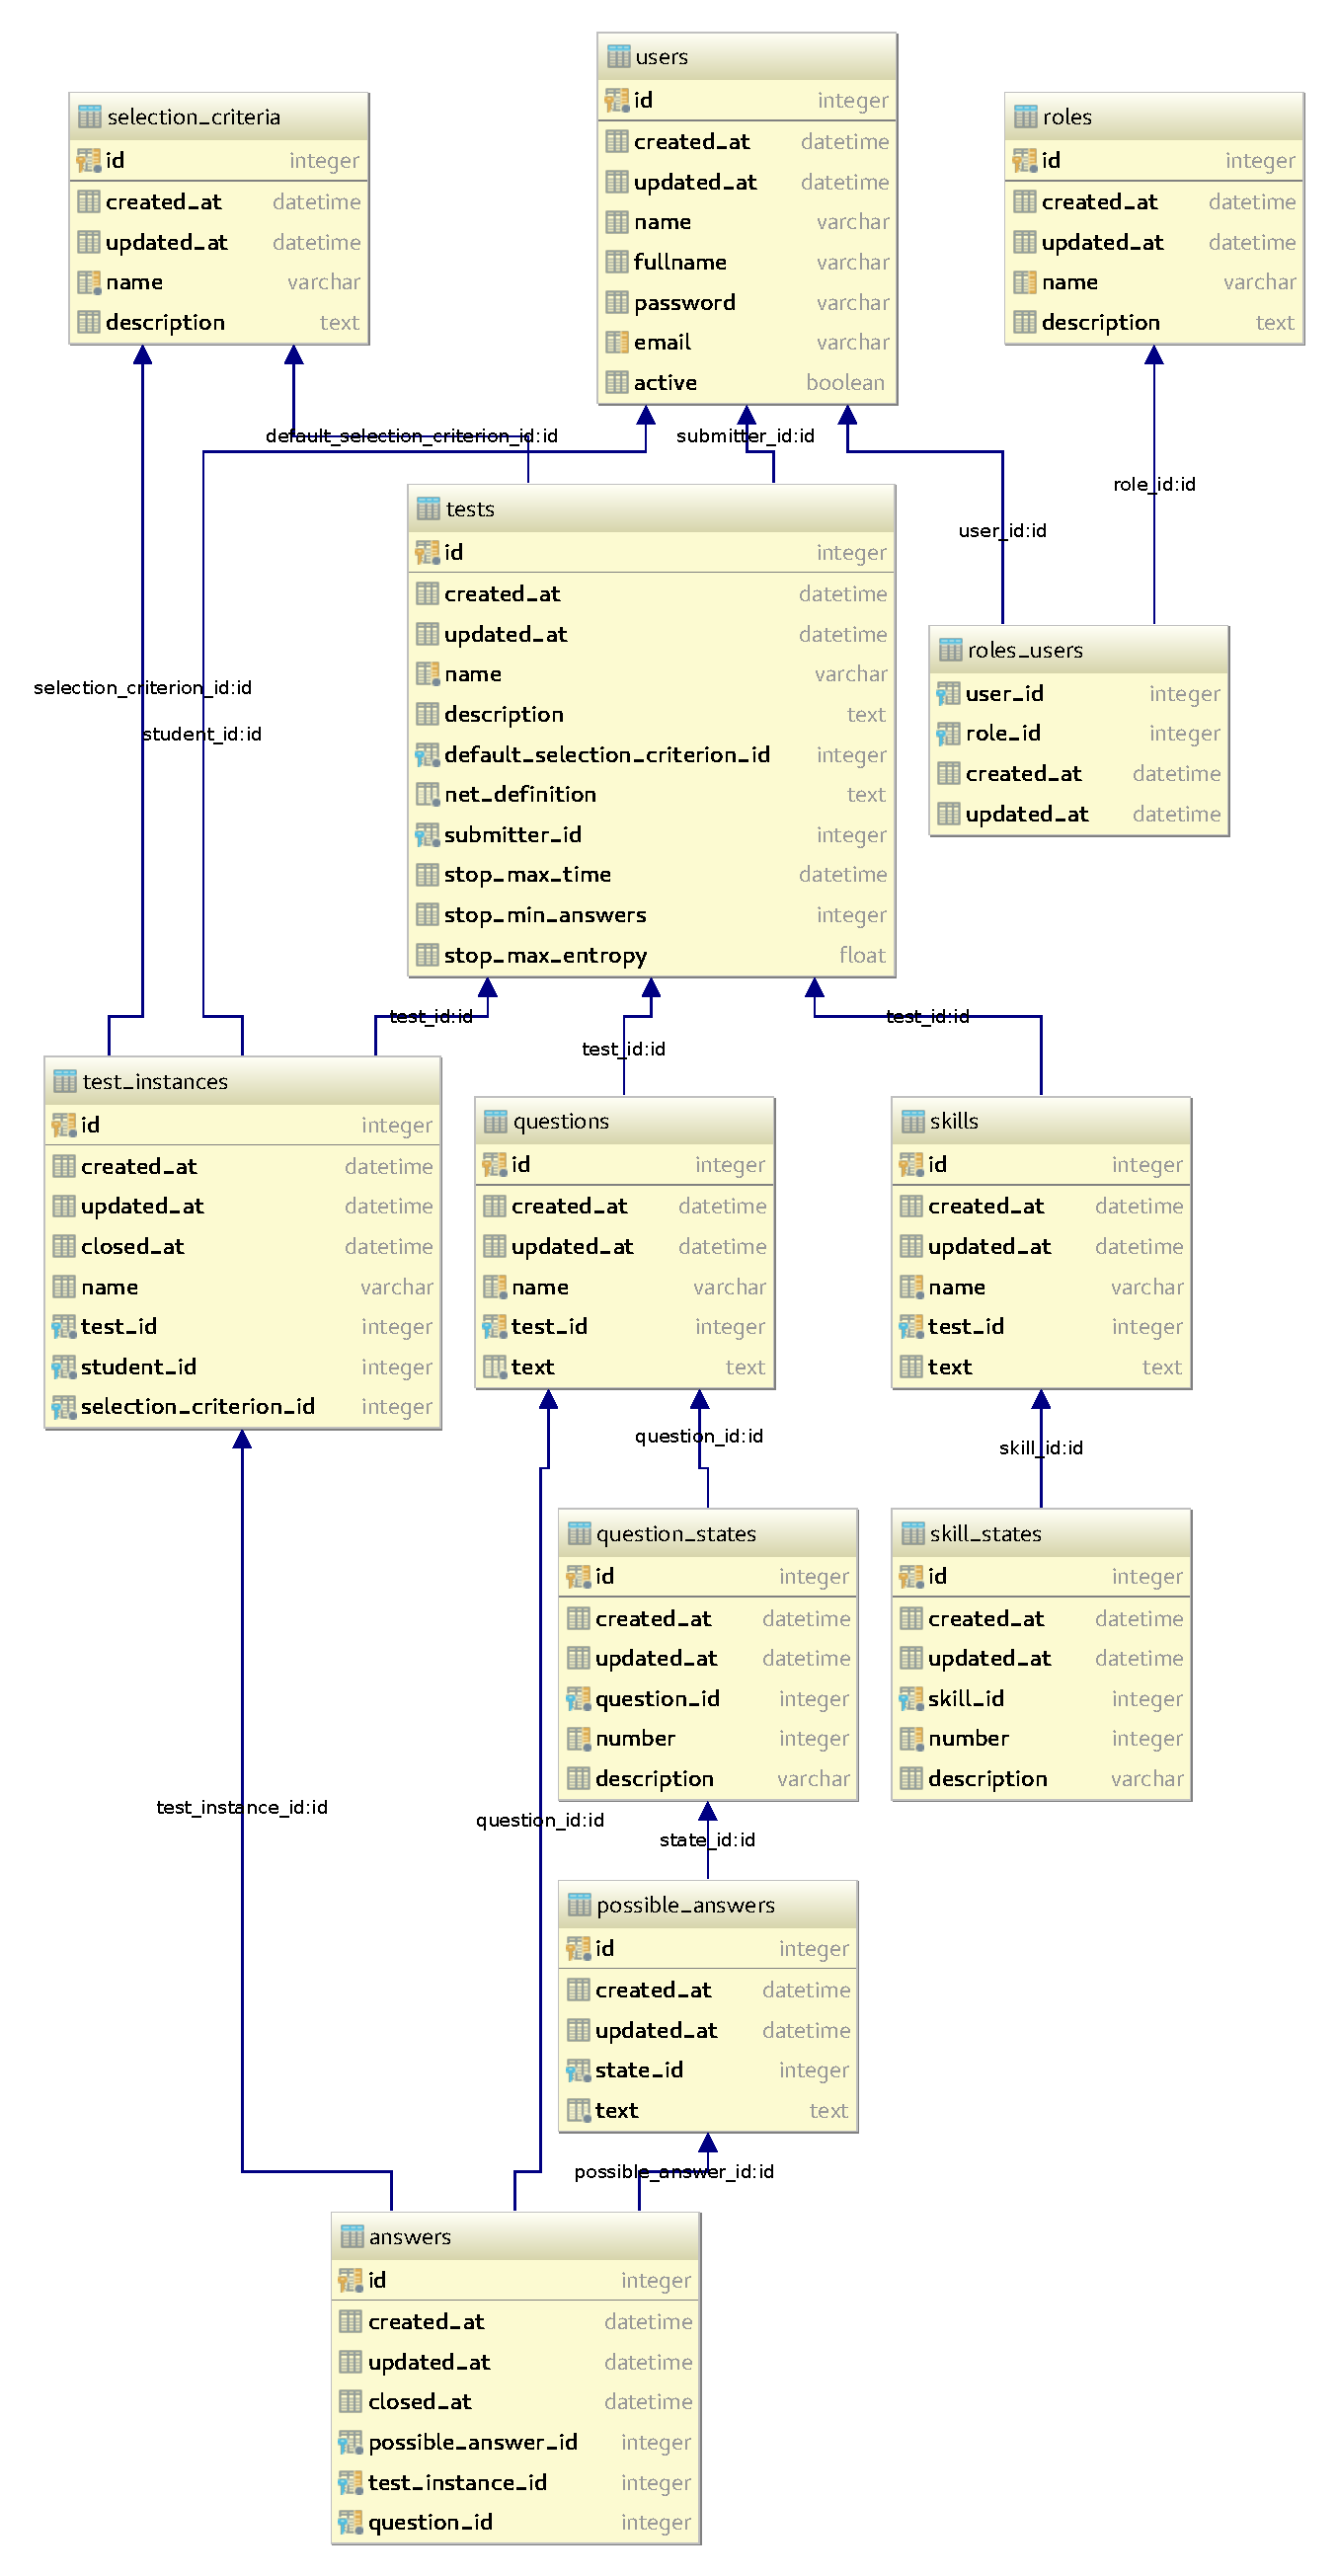
\includegraphics[width=0.75\textwidth]{data_model.pdf}
  \caption{Diagram datového modelu použitého v aplikaci. Jednotlivé rámečky reprezentují příslušné tabulky (resp. entity, případně třídy) a šipky vztahy mezi nimi (reference pomocí cizích klíčů).}
  \label{fig:data_model}
\end{figure}

Obecný význam entit (tabulek) a většiny jejich vlastností (sloupců) na obrázku \ref{fig:data_model} je asi zřejmý, ale raději zde dále alespoň zasadím do kontextu všechny tabulky.

Tabulky \texttt{users}, \texttt{roles} a \texttt{roles\_users} zaznamenávají identity uživatelů. Existenci tabulky pro role předpokládá knihovna \textit{Flask-Security}, která zajišťuje v aplikaci správu identit. Kdyby tomu tak nebylo, tabulka \texttt{roles} ani \texttt{roles\_users}, by se v modelu nevyskytla. \cite{Flask-Security}

Tabulka \texttt{tests} obsahuje informace o testu jako celku. Sloupec \texttt{net\_definition} obsahuje definici struktury sítě i tabulek podmíněných pravděpodobností ve formátu, který dokáže zpracovat knihovna \texttt{catest}. Konkrétně jde o textový formát, který pro ukládání používá aplikace \textit{Hugin Researcher} \cite{hugin}. Sloupec \texttt{stop\_max\_entropy} udává požadovanou úroveň (Shannonovy) entropie stavů dovedností v bitech, konkrétně počítané jako suma napříč dovednostmi:
\begin{equation}
	H(e) = -\sum_{S_i \in \mathcal{S}}\sum_{s_i \in \mathbb{S}_i}P(S_i=s_i|e) \log_2 P(S_i=s_i|e).
\end{equation}

Tabulky \texttt{questions} a \texttt{question\_states} slouží k záznamu otázek daného testu a jejich možných stavů, analogicky lze popsat tabulky \texttt{skills} a \texttt{skill\_states} (měřené dovednosti a jejich stavy). Sloupec \texttt{name} u otázek a dovedností slouží k identifikaci příslušného uzlu ve struktuře sítě, sloupec \texttt{number} zase k identifikaci stavu v tabulkách podmíněných pravděpodobností. Tyto tabulky lze částečně generovat na základě \texttt{net\_definition}, ale \texttt{net\_definition} neobsahuje samotný text otázek, ani popis jejich stavů, takže ten musí doplnit zadavatel zvlášť. Hodnoty ve sloupcích \texttt{name} a \texttt{number} musí odpovídat pojmenování, resp. číslu stavu, daného uzlu v \texttt{net\_definition}.

V tabulce \texttt{possible\_answers} se nacházejí možné odpovědi na otázky (které pak vedou na určítý stav otázky). Je tedy nutné, aby test sestával z uzavřených otázek (tedy otázek s předem danou sadou možných odpovědí). Tabulka \texttt{test\_instances} uchovává informace o jednotlivých případech testů a tabulka \texttt{answers} samotné odpovědi studenta na položené otázky.

Všechny tabulky obsahují sloupce \texttt{created\_at} a \texttt{updated\_at}, které uchovávají datum a čas vytvoření daného řádku v tabulce, resp. jeho poslední změny. Tabulky \texttt{test\_instances} a \texttt{answers} navíc obsahují sloupec \texttt{closed\_at}, který udává časovou značku uzavření daného případu testu nebo odpovědi. Tyto záznamy jsou užitečné pro kopírování záznamů do jiných databází: vždy stačí kopírovat jen záznamy, které vznikly nebo byly změněny po času posledního kopírování. Tyto časové údaje mohou také být užitečné pro analýzu dat, třeba pro odhad doby řešení otázek apod.

Při deklaraci datového modelu jsem navíc i nastavil indexování některých sloupců, resp. jejich kombinací (pro zrychlení vyhledávání), a integritní omezení, na příklad to, že v tabulce \texttt{skills} musí být kombinace \texttt{test\_id} a \texttt{name} unikátní.

Složitější operace nad datovým modelem jsou naprogramovány jako funkce v souboru \texttt{/datamodel/procedures.py}.

\begin{listing}
\centering
\begin{minted}[linenos,fontsize=\footnotesize]{python}
class TimeStampMixin:
    created_at: datetime = Column(DateTime, default=_get_date)
    updated_at: datetime = Column(DateTime, onupdate=_get_date)


class Skill(ModelBase, TimeStampMixin):
    __tablename__ = 'skills'

    id: int = Column(Integer, primary_key=True, index=True)
    name: str = Column(String, nullable=False)
    test_id: int = Column(Integer, ForeignKey('tests.id'), nullable=False)
    text: str = Column(Text)

    test: Test = relationship("Test", back_populates="skills")
    states: List[SkillState] = relationship("SkillState", back_populates="skill")

    __table_args__ = (UniqueConstraint('name', 'test_id', name='_test_skill_name_ux'),)
\end{minted}
\caption{Definice \uv{mixinu} pro časovou značku vytvoření a poslední změny a deklarace třídy pro dovednnost z \texttt{datamodel/model.py}.}
\label{lst:SkillDeclaration}
\end{listing}

\subsection{Rozhraní s \textit{R}}
V této sekci krátce popíšu svoji konkrétní implementaci rozhraní mezi \textit{Pythonem} a \textit{R}. Celé toto rozhraní je naprogramováni v modulu \texttt{inteRface}.

Potřebné funkce z \texttt{catest} jsou volány v souboru \texttt{/inteRface/procedures.py}. Bylo nutné, abych si doprogramoval v \textit{R} i dvě pomocné funkce -- jsou uvedeny přímo v tomto souboru.

Od těchto implementačních detailů je ovšem zbytek aplikace odstíněn pomocí abstrakce v podobě třídy \mintinline{python}|BayesNet| v souboru \texttt{/inteRface/classes.py}. Pomocí operací na objektech této třídy lze provádět všechny potřebné interakce s knihovnou \texttt{catest}, konkrétně jde o zpracování textových definic bayesovských sítí, vkládání informací do modelu, výběr otázek a získávání pravděpodobností stavů dovedností (což jsou v podstatě výsledky testu).

\begin{listing}
\centering
\begin{minted}[linenos,fontsize=\footnotesize]{python}
ro.r('''get.numbers.of.states <- function(model, node_vector) {
                nl <- model@nodes[node_vector]
                vv <- 1:length(nl@nodes)
                for(node in 1:length(nl@nodes)){
                    vv[node] <- nl@nodes[[node]]@number.of.states
                }
                vv
            }''')
r_get_numbers_of_states = ro.r['get.numbers.of.states']
\end{minted}
\caption{Funkce v \textit{R} zahrnuté v kódu \textit{Pythonu} z \texttt{inteRface/procedures.py}.}
\label{lst:PyR}
\end{listing}

Vzhledem k tomu, že šlo o asi nejkomplikovanější část aplikace na implementaci, napsal jsem k modulu \texttt{inteRface}, konkrétně ke třídě \mintinline{python}|BayesNet|, jednotkové testy do souboru \texttt{/dev/test\_bayesNet.py}.

\subsection{Webové rozhraní}
Samotnou interakci s uživatelem zajišťuje webové rozhraní. HTTP požadavky od uživatelů jsou obslouženy funkcemi definovanými v souboru \texttt{routing.py}. Pro názornost zde jednu uvedu a popíšu.

\begin{listing}
\centering
\begin{minted}[linenos,fontsize=\footnotesize]{python}
@app.route('/test/<int:test_id>')
@login_required
def test_overview(test_id):
    test: Test = get_entity_by_type_and_id(Test, test_id)
    check_test_existence_and_redirect_if_not_exists(test)
    test_instances = list_test_instances_by_test_and_student(test, current_user)
    possible_criteria = list_selection_criteria()
    test_instance_options_form = \
      TestInstanceOptionsForm(possible_criteria=[(sc.id, sc.name) for sc
			                         in possible_criteria],
                              default_criterion=test.default_selection_criterion.id)
    return render_template("test_overview.html", test=test,
		           test_instances=test_instances,
                           test_instance_options_form=test_instance_options_form,
                           possible_criteria=possible_criteria)

\end{minted}
\caption{Funkce pro zobrazení přehledu testu z \texttt{routing.py}.}
\label{lst:test_view}
\end{listing}

Na prvních dvou řádcích v ukázce kódu \ref{lst:test_view} jsou tak zvané dekorátory. První z nich zajišťuje propojení s příslušnou URI požadavku -- argument dekorátoru je URI s tím, že pomocí podřetězce \mintinline{python}|<int:test_id>| je určeno, že na konci URI má být číslo, které se má pak dekorované funkci předat jako argument. Druhý dekorátor zajišťuje, že pro zobrazení stránky je nutné, aby byl uživatel přihlášen. Provedením řádku 4 se do proměnné \mintinline{python}|test| nahraje objekt reprezentující test (třída je anotována dle \cite{PEP484}). Následuje kontrola, že test vůbec v databázi existuje (pokud ne, je uživatel přesměrován na seznam testů). Poté jsou do příslušných proměnných nahrány případy daného testu, výběrová kritéria a formulář pro zahájení nového případu testu. Nakonec funkce vrátí \uv{vykreslenou} šablonu \mintinline{python}|"test_overview.html"|.

Ostatní funkce definované v \texttt{routing.py} mají podobnou strukturu. Nejdříve se načtou do proměnných data z databáze, proběhne kontrola vstupů (fragmenty URI jako \mintinline{python}|test_id| výše a případně data z formulářů), jsou provedeny změny v databázi, je-li to třeba, nakonec je buď \uv{vykreslena} příslušná šablona a odeslána uživateli, nebo je uživatel někam přesměrován.

Šablony se vykreslují pomocí systému \textit{Jinja} \cite{jinja2}. Všechny šablony jsou ve složce \texttt{templates}. Základní šablona (všechny ostatní jsou od ní odvozeny) tvoří soubor \texttt{common.html}, který také slouží jako šablona pro úvodní stránku.

Celá struktura používaných URI je navržena, jako kdyby šlo o REST API. Dokonce platí, že požadavky, které způsobují tvorbu nových záznamů v databázi musejí používat HTTP metodu \texttt{POST} (všude jinde se předpokládá metoda \texttt{GET}).

Tvorbu a validaci formulářů zajišťuje knihovna \textit{WTForms} \cite{wtforms}. Také asi stojí za zmínku, že samotný web (tedy příslušný HTML a CSS kód) je psán pomocí CSS šablony \textit{Skeleton} \cite{skeleton.css}, díky které je \uv{responzivní}, tedy měl by být použitelný i na mobilních zařízeních (telefony, tablety apod.).

Funkce pro vyřizování HTTP požadavků používají k přístupu k datovému modelu různé pomocné funkce a třídu \mintinline{python}|BayesNetDataModelWrapper| z modulu \texttt{common}. Třída \mintinline{python}|BayesNetDataModelWrapper| zapouzdřuje je jakýmsi pomyslným těžištěm aplikace, protože integruje operace v rámci \texttt{catest} s operacemi na datech v databázi. Pomocí metod této třídy protékají data mezi databází a \textit{R}, případně nakonec i k uživateli jako hypertext.

\section{Pracovní postup studenta}
Student může začít na úvodní stránce, nebo může být odkázán přímo na požadovaný test (třeba \url{http://cat.utia.cas.cz:1080/test/1}). Poté by měl zahájit nový případ testu.
% TODO: link shoud work as expected, update app on server

Po zahájení případu testu začne běžet čas testu (což je relevantní, pokud je nastavena nějaká maximální doba řešení testu). Student si může otázku vybrat sám ze seznamu, nebo využít možnosti automatického výběru dle kritéria.

Jakmile je dosaženo nějakého z ukončovacích kritérií (entropie na dovednostech klesne pod zadanou mez, je zodpovězen dostatečný počet otázek, nebo uplyne vyhrazený čas), je případ testu uzavřen. Výsledky v podobě pravděpodobností stavů dovednostních veličin jsou průběžně zobrazovány v přehledu případu testu.

\section{Analýza časové náročnosti}
Analyzoval jsem zběžně časovou náročnost operací nutných pro chod aplikace. Nejvíce uživatel vždy pocítí, pokud je k vyřízení jeho poždavku nutné použít \texttt{catest}. Nejvíce času v tomto případě aplikace stráví výpočty v rámci této knihovny. Sám vedoucí práce uvedl, že se při vývoji autoři \texttt{catest} nesnažili příliš optimalizovat časovou náročnost. Problémem je i fakt, že v \textit{R} se zpravidla argumenty funkcí předávají kopírováním, což samozřejmě značně zvyšuje paměťové i výpočetní nároky.

Tyto problémy by šlo řešit třeba tak, že by se po zodpovězení otázky asynchronně (než student zodpoví další otázky) uvažovaly všechny možné scénáře vývoje testu několik dalších kroků testu dopředu. Tyto scénáře i s příslušnými otázkami by se zazamenávaly do databáze a výběr otázky by pak znamenal jen vyhledání v databázi. Také by samozřejmě bylo možné provést alternativní implementaci funkcionality \texttt{catest}, která by byla výrazně rychlejší třeba v \textit{C++} nebo \textit{Julia} \cite{julia}. Další možností vývoje uvedu v následující sekci.
% TODO: změnit strukturu druhé kapitoly

\section{Možnosti budoucího vývoje}
Největším problémem aplikace je, že užvatelské rozhraní nemá žádné nástroje pro analýzu výsledků testu (tedy aspoň nic komplexnějšího než prosté zobrazení pravděpodobností stavů dovedností). Nicméně dat o průběhu testů systém shromažďuje, dle mého názoru, dostatek, rozvoj je v tomto směru tedy možný dosti velký.

Celkově by asi bylo na místě vyvinou nějaké vlastní webové rozhraní pro zadávání a administraci testů. Zatím by bylo nejjednodušší pro zadávání testů do systému navrhnout nějaký strojově čitelný formát založený třeba na XML, nebo i prostý XML soubor či JSON.

Co se týče hlubší analýzy výsledků, mělo by asi smysl uvažovat na příklad o analýze častých sledů otázek, korelace stavů otázek, rychlost poklesu entropie v modelu (nebo v jeho částech) nebo třeba o nějakém souhrnu výsledků daného testu (třeba histogram pravděpodobností stavů).

% -------------------------------------
\chapter*{Závěr} % SEM NESAHEJTE!
\addcontentsline{toc}{chapter}{Závěr} % SEM NESAHEJTE!

V první kapitole jsem krátce uvedl koncept adaptivního počítačového testování a popsal jsem krátce i možnosti jeho realizace pomocí bayesovských sítí. Na příkladu jsem popsal návrh adaptivního testu a popsal jsem několik strategií pro výběr otázek.

V druhé kapitole jsem popsal aplikaci, kterou jsem v rámci výzkumného úkolu vyvíjel a její vztah k systému pro adaptivní testování, vyvíjeného na Ústavu teorie informace a automatizace AV ČR, do kterého zapadá. Vysvětlil jsem výběr nástrojů, které jsem zvolil pro implementaci a popsal strukturu aplikace.

Aplikace nyní neposkytuje, byť to požadovalo zadání, žádné komplexní analytické výstupy. Na druhou stranu zadání specifikovalo, že by aplikace měla sloužit k testování znalostí studentů středních škol v oblasti matematiky, vyvinul jsem ovšem systém, který nepředpokládá žádnou konkrétní doménu znalostí k testování, pokud je možné otázky koncipovat výhradně jako uzavřené otázky.

Za největším přínos samotného textu považuji snad přiměřeně podrobnou dokumentaci systému. V textu je také uvedeno několik návrhů pro další vývoj aplikace třeba v rámci navazující diplomové práce.

%
%\input{vnitrek_zaver.tex}


%%%%%%%%%%%% SEZNAM POUŽITÝCH ZDROJŮ (LITERATURA) %%%%%%%%%%%%
\clearpage  % SEM NESAHEJTE!
\addcontentsline{toc}{chapter}{Literatura} % SEM NESAHEJTE!

\begin{thebibliography}{99}
	% formát: ČSN ISO 690. Můžete si to vygenerovat na http://www.citacepro.com (přihlaste se přes odkaz "ČVUT"), umí to vygenerovat TeX
	% řazení: abecedně podle autora (resp. prvního slova, není-li znám autor)
	\bibitem{almond_tlustospis} ALMOND, R.G., MISLEVY, R.J., STEINBERG, L., YAN, D., WILLIAMSON, D. \textit{Bayesian Networks in Educational Assessment.} Springer, 2015.

	\bibitem{vomlel_obec} VOMLEL, Jiří \textit{Bayesian networks in educational testing.} International Journal of Uncertainty, Fuzziness and Knowledge Based Systems. Vol. 12, Supplementary Issue 1, 2004, pp. 83-100.

	\bibitem{vomlel_building} VOMLEL, Jiří \textit{Building Adaptive Tests using Bayesian networks.} Kybernetika. Volume 40, Number 3, 2004, pp. 333 - 348.

	\bibitem{plajner16} PLAJNER, Martin, Jiří VOMLEL. \textit{Student Skill Models in Adaptive Testing.} Proceedings of the Eighth International Conference on Probabilistic Graphical Models, pp. 403–414, 2016.

% ------------------------

	\bibitem{Jensenc2007} JENSEN, Finn V. a Thomas D. NIELSEN. \textit{Bayesian networks and decision graphs}. 2nd ed. New York: Springer, c2007. ISBN 978-0-387-68282-2.

	\bibitem{Wainer2000} WAINER, Howard. a Neil J. DORANS. \textit{Computerized adaptive testing: a primer}. 2nd ed. Mahwah, N.J.: Lawrence Erlbaum Associates, 2000. ISBN 08-058-3511-3.

	\bibitem{vomlel_plajner2015} PLAJNER, Martin, Jiří VOMLEL. \textit{Bayesian network models for adaptive testing.} Proceedings of the Twelfth UAI Conference on Bayesian Modeling Applications Workshop-Volume 1565. CEUR-WS. org, 2015. p. 24-33.

	\bibitem{question_selection} PLAJNER, Martin, Amal MAGAUINA a Jiří VOMLEL. \textit{Question Selection Methods for Adaptive Testing with Bayesian Networks}. Ústav teorie informace a automatizace, Akademie věd České republiky, 2017.

% --------------------------------------

	\bibitem{R} \textit{R: The R Project for Statistical Computing} [online]. Vídeň: The R Foundation for Statistical Computing, 2017 [cit. 2017-08-31]. Dostupné z: https://www.r-project.org/

	\bibitem{python} \textit{Python} [online]. Beaverton: Python Software Foundation, 2017 [cit. 2017-08-31]. Dostupné z: https://www.python.org/

	\bibitem{r_shiny} \textit{R Shiny} [online]. Boston: RStudio, 2017 [cit. 2017-08-30]. Dostupné z: https://shiny.rstudio.com/

	\bibitem{flask} \textit{Flask: A python microframework} [online]. Pocoo Team, 2017 [cit. 2017-08-31]. Dostupné z: http://flask.pocoo.org/

	\bibitem{rpy2} \textit{RPy2} [online]. Laurent Gautier et al., 2017 [cit. 2017-08-31]. Dostupné z: https://rpy2.readthedocs.io

	\bibitem{sqlalchemy} \textit{SQLAlchemy: The database toolkit for Python} [online]. 2017 [cit. 2017-08-31]. Dostupné z: http://www.sqlalchemy.org/

	\bibitem{sqlite} \textit{SQLite} [online]. 2017 [cit. 2017-08-31]. Dostupné z: https://www.sqlite.org

	\bibitem{babel} \textit{Babel} [online]. Babel Team, c2017 [cit. 2017-08-30]. Dostupné z: http://babel.pocoo.org/en/latest/

	\bibitem{Flask-Security} \textit{Flask-Security} [online]. Matt Wright, c2012 [cit. 2017-08-31]. Dostupné z: https://pythonhosted.org/Flask-Security/

	\bibitem{wtforms} \textit{WTForms} [online]. WTForms Team, c2010 [cit. 2017-08-31]. Dostupné z: http://wtforms.readthedocs.io/

	\bibitem{jinja2} \textit{Jinja2} [online]. Armin Ronacher, c2014 [cit. 2017-08-31]. Dostupné z: http://jinja.pocoo.org/

	\bibitem{skeleton.css} \textit{Skeleton: Responsive CSS boilerplate} [online]. Dave Gamache et al., 2014 [cit. 2017-08-31]. Dostupné z: http://getskeleton.com/

	\bibitem{hugin} \textit{HUGIN} [online]. Aalborg: HUGIN EXPERT, 2017 [cit. 2017-08-31]. Dostupné z: http://www.hugin.com/

% ---------------------------------------

	\bibitem{ORM} Object-relational mapping. In: \textit{Wikipedia: the free encyclopedia} [online]. San Francisco (CA): Wikimedia Foundation, 2001- [cit. 2017-08-30]. Dostupné z: https://en.wikipedia.org/wiki/Object-relational\_mapping

	\bibitem{multiparadigm} Comparison of multi-paradigm programming languages. In: \textit{Wikipedia: the free encyclopedia} [online]. San Francisco (CA): Wikimedia Foundation, 2001-2017 [cit. 2017-08-30]. Dostupné z: https://en.wikipedia.org/w/index.php?title=Comparison\_of\_multi-paradigm\_programming\_languages\&oldid=797311914

	\bibitem{PEP484} PEP 484: Type Hints. \textit{Python} [online]. Python Foundation, 2014 [cit. 2017-08-31]. Dostupné z: https://www.python.org/dev/peps/pep-0484/

	\bibitem{CPython} CPython. In: \textit{Wikipedia: the free encyclopedia} [online]. San Francisco (CA): Wikimedia Foundation, 2017 [cit. 2017-09-07]. Dostupné z: https://en.wikipedia.org/w/index.php?title=CPython\&oldid=797221729

	\bibitem{julia} \textit{Julia Language} [online]. Austin: NumFocus, 2017 [cit. 2017-08-31]. Dostupné z: https://julialang.org/

\end{thebibliography}


%%%%%%%%%%%% PŘÍLOHY PRÁCE %%%%%%%%%%%%
\newpage % SEM NESAHEJTE!
\addcontentsline{toc}{chapter}{Přílohy} % SEM NESAHEJTE!
\appendix % SEM NESAHEJTE!


%%%%%%%%%%%% Příloha A (tj. 1. kapitola v rámci příloh) %%%%%%%%%%%%

\section*{Instalace a rozhraní přes příkazový řádek}
\label{appendix:installation}
\addcontentsline{toc}{section}{Instalace a rozhraní přes příkazový řádek}

V této sekci krátce popíšu možný postup instalace systému pro vyzkoušení. Budu zde předpokládat instalaci na nějakou moderní distribuci \textit{GNU/Linux} (třeba \textit{Fedora}, \textit{CentOS}, \textit{ArchLinux}, \textit{Antegros}). Dále uvedu několik příkazů, které aplikace podporuje (ze souboru \texttt{cli.py}).

Nejdříve je nutné zajistit, že jsou nainstalovány všechny závislosti. Vzhledem k tomu, že, jak jsem zmínil výše, používám typové anotace \cite{PEP484}, je nutné mít nainstalovaný \textit{Python} verze aspoň \texttt{3.5}. Pro chod knihovny \textit{RPy2} je naneštěstí nutné používat interpreter \textit{CPython} \cite{CPython}. Dále je potřeba mít nainstalovanou dostatečně novou verzi interpreteru \textit{R} (v moment psaní mám nainstalovanou verzi \texttt{3.4.1}). Také je potřeba mít k dispozici nějaký relační databázový systém. Bez zásahu do \texttt{CArisTotle/config}

Nejjednodušší asi je si naklonovat repozitář na \url{https://github.com/FNj/CArisTotle} a přesunout se do příslušné složky pomocí:
\begin{minted}{bash}
git clone https://github.com/FNj/CArisTotle
cd CArisTotle
\end{minted}
poté, byť to není nezbytně nutné, je vhodné vytvořit si pro aplikaci virtuální prostředí \textit{Pythonu}
Poté je potřeba nainstalovat knihovnu \texttt{catest} a další knihobny \textit{R}, na kterých je závislá. Vše potřebné je ve složce \texttt{dependencies/R}. Stačí si spustit interpreter (příkaz \mintinline{bash}|R|) a zadat příkaz:
\begin{minted}{R}
source("dependencies/R/install_deps.R")
\end{minted}
Budete vyzvání k výberu repozitáře, ze kterého se mají příslušné balíčky nainstalovat. Taky se pak nelekněte spousty varování compileru \textit{C++}.

Poté, byť to není nezbytně nutné, je vhodné vytvořit si pro aplikaci virtuální prostředí \textit{Pythonu} třeba jako:
\begin{minted}{bash}
python3 -m venv VEnv
\end{minted}
a aktivovat si ho:
\begin{minted}{bash}
source VEnv/bin/activate
\end{minted}

Následně si nainstalujte potřebné knihovny \textit{Pythonu}:
\begin{minted}{bash}
pip install -r requirements.txt
\end{minted}

Poté už lze začít používat samotnou aplikaci. Nejdříve je potřeba nastavit proměnnou ukazující na modul s aplikací:
\begin{minted}{bash}
export FLASK_APP=CArisTotle/__init__.py
\end{minted}
dále je potřeba inicializovat databázi (vytvoření schéma, naplnění číselníkových tabulek):
\begin{minted}{bash}
flask initdb
\end{minted}
pak je pro testování nutné naplnit databázi i testovacími daty:
\begin{minted}{bash}
flask testdata
\end{minted}
a teď už lze aplikaci spustit:
\begin{minted}{bash}
flask run
\end{minted}

Až skončíte práci s aplikací, můžete databázi snadno promazat:
\begin{minted}{bash}
flask dropall
\end{minted}

Pro nahrávání testů lze použít třeba skript podobný tomu v souboru \texttt{CArisTotle/dev/test_data.py}

\end{document} % SEM NESAHEJTE! Konec.
